79. \begin{figure}[ht!]
\center{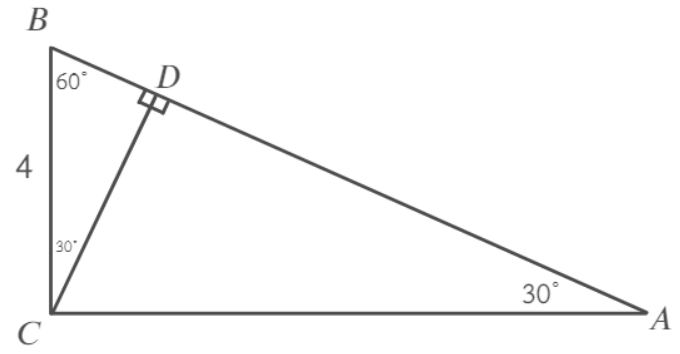
\includegraphics[scale=0.35]{g79.png}}
\end{figure}\\
В прямоугольном треугольнике $BCD$ катет $BD$ в 2 раза меньше гипотенузы $BC,$ значит $\angle BCD=30^\circ,\ \angle B=90^\circ-30^\circ=60^\circ,\ \angle A=90^\circ-60^\circ=30^\circ.$ Тогда по теореме о катете, лежащем напротив угла в $30^\circ,$ для треугольников $BCD$ и $ABC$ имеем $BD=4:2=2,\ AB=2\cdot4=8,$ значит  $AD=8-2=6.$\\
